\documentclass[a4paper,12pt, headsepline]{scrartcl}

\usepackage[utf8]{inputenc}
\usepackage[T1]{fontenc}
\pagestyle{plain}
\usepackage{lmodern}
\usepackage[english]{babel}
\usepackage[official]{eurosym}
\usepackage{ntheorem}
\newtheorem{hyp}{Hypothesis}
\usepackage{pdfpages}
\usepackage{adjustbox}
\usepackage{footnote}
\usepackage{filecontents}
\usepackage{titling}
\usepackage{csquotes}
\usepackage[objectset = centering]{floatrow}
\usepackage{moreverb}
\usepackage{varioref}
\usepackage{setspace}
\usepackage{graphicx}
\usepackage{tabularx}
\usepackage{dcolumn}
\usepackage{float}
\usepackage{color}
\usepackage{amsmath} 
\usepackage{float}
\usepackage[
colorlinks = true,
linkcolor = black,
citecolor = blue 
]{hyperref}


\setlength{\parindent}{0ex} 
\setlength{\parskip}{1ex}


\usepackage[automark]{scrlayer-scrpage}
\setkomafont{pagehead}{\scshape}
\pagestyle{scrheadings}
\ihead{\headmark}
\chead{}
\ohead{}

\cfoot{\pagemark}


\usepackage{csquotes}
\usepackage[
backend=biber,
natbib=true,
language = english,
doi = false, url = false, isbn = false, eprint = false,
style = apa]
{biblatex}
\DeclareLanguageMapping{english}{english-apa}
\addbibresource{literature.bib}

% Schrift
\setkomafont{sectioning}{\rmfamily\bfseries\boldmath}

\setcapindent{0em} % kein Einrücken der Caption von Figures und Tabellen
\setcapwidth{0.9\textwidth} % Breite der Caption nur 90% der Textbreite, damit sie sich vom restlichen Text abhebt
\setlength{\abovecaptionskip}{0.2cm} % Abstand der zwischen Bild- und Bildunterschrift
\renewcommand{\baselinestretch}{1.5}
\numberwithin{equation}{section}
\title{Predicting Award Prices of First Price Sealed Bid Procurement Auctions}
\date{07/14/2022}
\author{Fabian Blasch\\[0.4cm]{Supervisor: Dr. Katharina Fenz}}
\begin{document}
\begin{titlingpage}
\maketitle
\end{titlingpage}
\newpage
\tableofcontents
\newpage
\section{Introduction}\label{sec:int}

\section{Data}\label{sec:data}

All the information about the procurement contracts, is obtainable through the bid tab archive on the official website of the Colorado Department of Transportation. The information is provided in PDF documents. In each of those documents the following information of the respective auction is covered.

\begin{itemize}
	\item A table listing all submitted bids, including a unique identifier for each of the participating bidders
	\item An Engineer's Estimate
	\item The contract ID
	\item The letting date
	\item Either the amount of time in business days given to complete all the contracted obligations, or a completion due date
	\item The County in which the contract is to be completed in 
\end{itemize}

For illustrative, Figure \ref{fig:bidtab} displays an example of a bid tab, in particular the second page, which contains the vendor ranking as well as the contract description and the remaining information listed above.

\begin{figure}[H]
	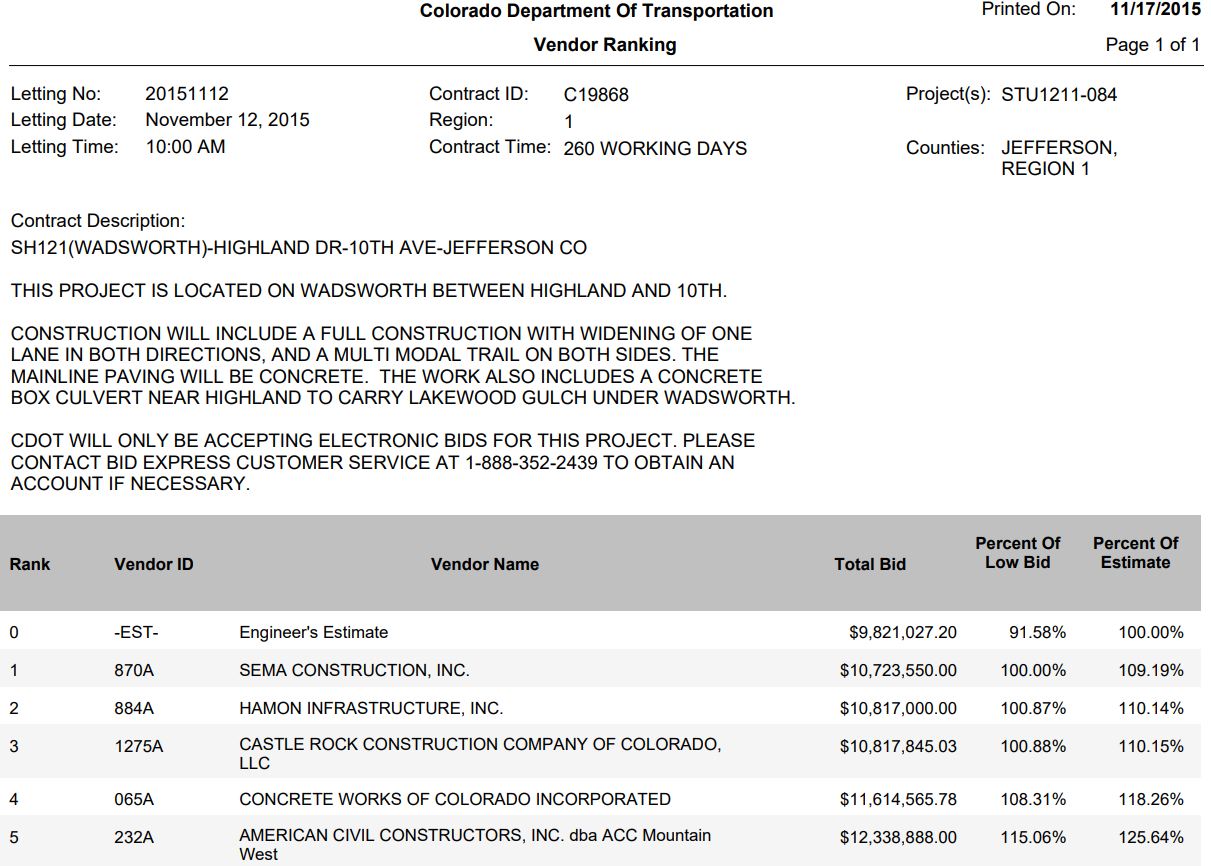
\includegraphics[width = 14	cm]{figures/Bid_Tab_exmpl.PNG}
	\caption{Bid Tab Example}\label{fig:bidtab}
\end{figure}

\subsection{Scraping}\label{subsec:scrap}
In order to obtain all the archived bid tabs, the html code of the website was first examined using a google chrome extension called SelectorGadget. This tool allows one to identify html nodes, that website contents are associated with. In the case of the bid tab archive, the html node carrying the links to the individual bid tabs is \enquote{<td a>}. Once this html node is discovered and the consistency across different years in the archive is ensured, the download is easily achieved by looping over the links and downloading the  respective PDF. The hyperlink extraction was performed utilizing \textit{rvest}, by \citet{rvest}. For the remaining steps in the data extraction, a distinction will be made for text based information and tabular data.

\subsubsection{Text Based Information}\label{subsubsec:descr}
 The structure of the text based information allows us to filter the individual parts via regular expressions. Especially, for the letting data, the contract ID, and the Counties this required no further data cleaning steps. Unfortunately, this is not the case for the contract time and the contract description. 
 
 
\begin{figure}[H]
	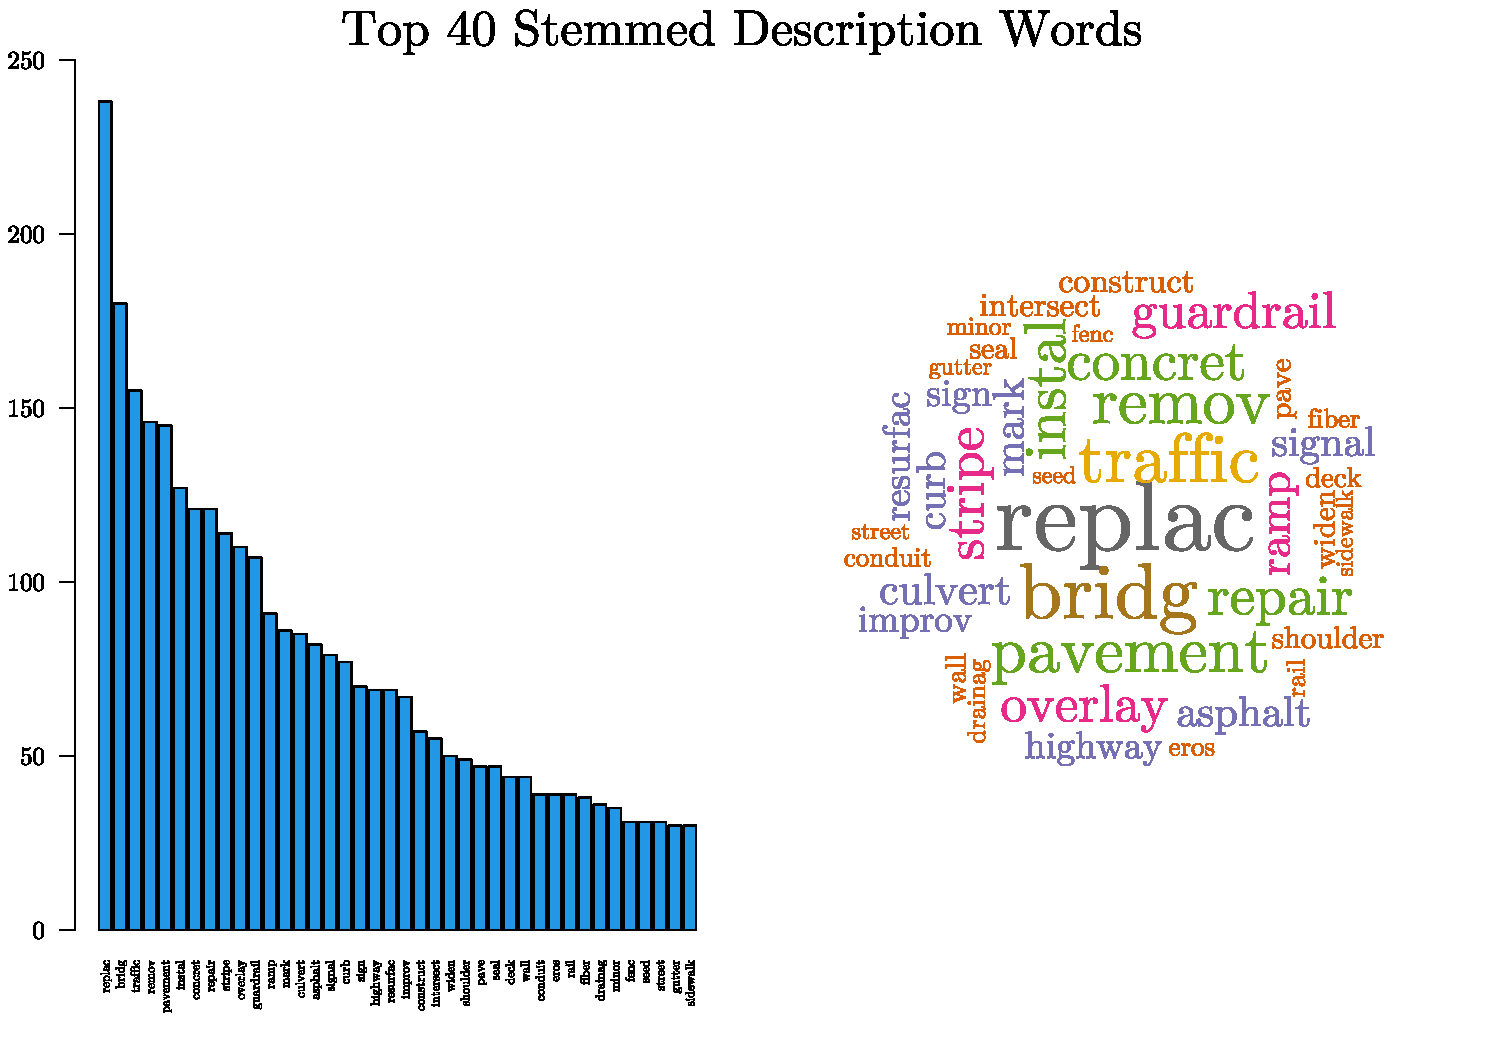
\includegraphics[width = 14	cm]{figures/description_words.pdf}
	\caption{Top 40 Stemmed Description Words}\label{fig:desc}
\end{figure}

\subsection{Descriptive Statistics}\label{subsec:desc}
\section{Economic Operationalization}\label{sec:op}
\subsection{Auctioneer}\label{subsec:auc}
\subsection{Firms}\label{subsec:firms}

\section{Methods}\label{sec:meth}
\subsection{Elastic Nets}\label{subsec:net}
\subsection{Ensemble Methods}\label{subsec:ens}
\subsubsection{Random Forests}\label{subsubsec:rf}
\subsubsection{eXtreme Gradient Boosting}\label{subsubsec:xgb}
\subsection{Nested Cross Validation}\label{subsec:nest}
\subsubsection{Logistic PCA}\label{subsubsec:logp}
\subsubsection{Recursive Feature Elimination}\label{subsubsec:rfe}
\section{Results}\label{sec:res}
\subsection{Prediction}\label{subsec:pred}
\subsection{Unsupervised Colusion Detection}\label{subsec:col}
\section{Conclusion}\label{sec:con}
 
\newpage
\printbibliography

\end{document}